% Options for packages loaded elsewhere
\PassOptionsToPackage{unicode}{hyperref}
\PassOptionsToPackage{hyphens}{url}
\PassOptionsToPackage{dvipsnames,svgnames,x11names}{xcolor}
%
\documentclass[
  10pt,
  ignorenonframetext,
]{beamer}
\usepackage{pgfpages}
\setbeamertemplate{caption}[numbered]
\setbeamertemplate{caption label separator}{: }
\setbeamercolor{caption name}{fg=normal text.fg}
\beamertemplatenavigationsymbolsempty
% Prevent slide breaks in the middle of a paragraph
\widowpenalties 1 10000
\raggedbottom
\setbeamertemplate{part page}{
  \centering
  \begin{beamercolorbox}[sep=16pt,center]{part title}
    \usebeamerfont{part title}\insertpart\par
  \end{beamercolorbox}
}
\setbeamertemplate{section page}{
  \centering
  \begin{beamercolorbox}[sep=12pt,center]{part title}
    \usebeamerfont{section title}\insertsection\par
  \end{beamercolorbox}
}
\setbeamertemplate{subsection page}{
  \centering
  \begin{beamercolorbox}[sep=8pt,center]{part title}
    \usebeamerfont{subsection title}\insertsubsection\par
  \end{beamercolorbox}
}
\AtBeginPart{
  \frame{\partpage}
}
\AtBeginSection{
  \ifbibliography
  \else
    \frame{\sectionpage}
  \fi
}
\AtBeginSubsection{
  \frame{\subsectionpage}
}
\usepackage{amsmath,amssymb}
\usepackage{lmodern}
\usepackage{setspace}
\usepackage{iftex}
\ifPDFTeX
  \usepackage[T1]{fontenc}
  \usepackage[utf8]{inputenc}
  \usepackage{textcomp} % provide euro and other symbols
\else % if luatex or xetex
  \usepackage{unicode-math}
  \defaultfontfeatures{Scale=MatchLowercase}
  \defaultfontfeatures[\rmfamily]{Ligatures=TeX,Scale=1}
\fi
% Use upquote if available, for straight quotes in verbatim environments
\IfFileExists{upquote.sty}{\usepackage{upquote}}{}
\IfFileExists{microtype.sty}{% use microtype if available
  \usepackage[]{microtype}
  \UseMicrotypeSet[protrusion]{basicmath} % disable protrusion for tt fonts
}{}
\makeatletter
\@ifundefined{KOMAClassName}{% if non-KOMA class
  \IfFileExists{parskip.sty}{%
    \usepackage{parskip}
  }{% else
    \setlength{\parindent}{0pt}
    \setlength{\parskip}{6pt plus 2pt minus 1pt}}
}{% if KOMA class
  \KOMAoptions{parskip=half}}
\makeatother
\usepackage{xcolor}
\geometry{left = 1cm, right = 0.5cm, top = 0.5cm, bottom = 0.5cm}
\newif\ifbibliography
\usepackage{color}
\usepackage{fancyvrb}
\newcommand{\VerbBar}{|}
\newcommand{\VERB}{\Verb[commandchars=\\\{\}]}
\DefineVerbatimEnvironment{Highlighting}{Verbatim}{commandchars=\\\{\}}
% Add ',fontsize=\small' for more characters per line
\usepackage{framed}
\definecolor{shadecolor}{RGB}{248,248,248}
\newenvironment{Shaded}{\begin{snugshade}}{\end{snugshade}}
\newcommand{\AlertTok}[1]{\textcolor[rgb]{0.94,0.16,0.16}{#1}}
\newcommand{\AnnotationTok}[1]{\textcolor[rgb]{0.56,0.35,0.01}{\textbf{\textit{#1}}}}
\newcommand{\AttributeTok}[1]{\textcolor[rgb]{0.77,0.63,0.00}{#1}}
\newcommand{\BaseNTok}[1]{\textcolor[rgb]{0.00,0.00,0.81}{#1}}
\newcommand{\BuiltInTok}[1]{#1}
\newcommand{\CharTok}[1]{\textcolor[rgb]{0.31,0.60,0.02}{#1}}
\newcommand{\CommentTok}[1]{\textcolor[rgb]{0.56,0.35,0.01}{\textit{#1}}}
\newcommand{\CommentVarTok}[1]{\textcolor[rgb]{0.56,0.35,0.01}{\textbf{\textit{#1}}}}
\newcommand{\ConstantTok}[1]{\textcolor[rgb]{0.00,0.00,0.00}{#1}}
\newcommand{\ControlFlowTok}[1]{\textcolor[rgb]{0.13,0.29,0.53}{\textbf{#1}}}
\newcommand{\DataTypeTok}[1]{\textcolor[rgb]{0.13,0.29,0.53}{#1}}
\newcommand{\DecValTok}[1]{\textcolor[rgb]{0.00,0.00,0.81}{#1}}
\newcommand{\DocumentationTok}[1]{\textcolor[rgb]{0.56,0.35,0.01}{\textbf{\textit{#1}}}}
\newcommand{\ErrorTok}[1]{\textcolor[rgb]{0.64,0.00,0.00}{\textbf{#1}}}
\newcommand{\ExtensionTok}[1]{#1}
\newcommand{\FloatTok}[1]{\textcolor[rgb]{0.00,0.00,0.81}{#1}}
\newcommand{\FunctionTok}[1]{\textcolor[rgb]{0.00,0.00,0.00}{#1}}
\newcommand{\ImportTok}[1]{#1}
\newcommand{\InformationTok}[1]{\textcolor[rgb]{0.56,0.35,0.01}{\textbf{\textit{#1}}}}
\newcommand{\KeywordTok}[1]{\textcolor[rgb]{0.13,0.29,0.53}{\textbf{#1}}}
\newcommand{\NormalTok}[1]{#1}
\newcommand{\OperatorTok}[1]{\textcolor[rgb]{0.81,0.36,0.00}{\textbf{#1}}}
\newcommand{\OtherTok}[1]{\textcolor[rgb]{0.56,0.35,0.01}{#1}}
\newcommand{\PreprocessorTok}[1]{\textcolor[rgb]{0.56,0.35,0.01}{\textit{#1}}}
\newcommand{\RegionMarkerTok}[1]{#1}
\newcommand{\SpecialCharTok}[1]{\textcolor[rgb]{0.00,0.00,0.00}{#1}}
\newcommand{\SpecialStringTok}[1]{\textcolor[rgb]{0.31,0.60,0.02}{#1}}
\newcommand{\StringTok}[1]{\textcolor[rgb]{0.31,0.60,0.02}{#1}}
\newcommand{\VariableTok}[1]{\textcolor[rgb]{0.00,0.00,0.00}{#1}}
\newcommand{\VerbatimStringTok}[1]{\textcolor[rgb]{0.31,0.60,0.02}{#1}}
\newcommand{\WarningTok}[1]{\textcolor[rgb]{0.56,0.35,0.01}{\textbf{\textit{#1}}}}
\setlength{\emergencystretch}{3em} % prevent overfull lines
\providecommand{\tightlist}{%
  \setlength{\itemsep}{0pt}\setlength{\parskip}{0pt}}
\setcounter{secnumdepth}{-\maxdimen} % remove section numbering
\usepackage[absolute,overlay]{textpos}
\usepackage{scalerel,stackengine}
\usepackage{everypage-1x}

\stackMath
\newcommand\reallywidehat[1]{%
\savestack{\tmpbox}{\stretchto{%
  \scaleto{%
    \scalerel*[\widthof{\ensuremath{#1}}]{\kern.1pt\mathchar"0362\kern.1pt}%
    {\rule{0ex}{\textheight}}%WIDTH-LIMITED CIRCUMFLEX
  }{\textheight}% 
}{2.4ex}}%
\stackon[-6.9pt]{#1}{\tmpbox}%
}

\newcommand\MyText[1]{%
  \begin{textblock*}{4.5cm}(0.7\textwidth,6cm)%
    #1
  \end{textblock*}
}
\usepackage{float}
\usepackage{booktabs}
\usepackage{array}
\usepackage{multirow}
\usepackage{mathtools}
\usepackage{xcolor}
\setbeamertemplate{itemize item}{$\diamond$}
\setbeamertemplate{itemize subitem}{\scriptsize$\diamond$}
\setbeamertemplate{navigation symbols}{}
\setbeamertemplate{footline}[page number]
\definecolor{blue}{RGB}{0,114,178}
\definecolor{red}{RGB}{213,94,0}
\definecolor{yellow}{RGB}{240,228,66}
\definecolor{green}{RGB}{0,158,115}
\ifLuaTeX
  \usepackage{selnolig}  % disable illegal ligatures
\fi
\IfFileExists{bookmark.sty}{\usepackage{bookmark}}{\usepackage{hyperref}}
\IfFileExists{xurl.sty}{\usepackage{xurl}}{} % add URL line breaks if available
\urlstyle{same} % disable monospaced font for URLs
\hypersetup{
  pdftitle={Econometrics: Multiple Regression and Applications},
  pdfauthor={Duong Trinh},
  colorlinks=true,
  linkcolor={blue},
  filecolor={Maroon},
  citecolor={Blue},
  urlcolor={Blue},
  pdfcreator={LaTeX via pandoc}}

\title{Econometrics: Multiple Regression and Applications}
\subtitle{ECON4004: LAB 4}
\author{Duong Trinh}
\date{February 28, 2024}
\institute{University of Glasgow}

\begin{document}
\frame{\titlepage}

\setstretch{1.5}
\begin{frame}{Intro}
\protect\hypertarget{intro}{}
\begin{itemize}
\tightlist
\item
  Duong Trinh

  \begin{itemize}
  \tightlist
  \item
    PhD Student in Economics (Bayesian Microeconometrics)
  \item
    Email: \underline{Duong.Trinh@glasgow.ac.uk}
  \end{itemize}
\end{itemize}

\vspace{3mm}

\begin{itemize}
\tightlist
\item
  ECON4004-LB01

  \begin{itemize}
  \tightlist
  \item
    Wednesday 10am -12 pm
  \item
    5 sessions (7-Feb, 14-Feb, 21-Feb, 28-Feb, 6-March)
  \item
    ST ANDREWS:357
  \end{itemize}
\item
  ECON4004-LB02

  \begin{itemize}
  \tightlist
  \item
    Wednesday 12-2 pm
  \item
    5 sessions (7-Feb, 14-Feb, 21-Feb, 28-Feb, 6-March)
  \item
    ST ANDREWS:357
  \end{itemize}
\end{itemize}
\end{frame}

\begin{frame}{Record Attendance}
\protect\hypertarget{record-attendance}{}
\end{frame}

\begin{frame}{Plan for LAB 4}
\protect\hypertarget{plan-for-lab-4}{}
\begin{itemize}
\tightlist
\item
  Exercise 1: based on Stock \& Watson, E10.1
\item
  Exercise 2: based on Stock \& Watson, E10.2
\end{itemize}

\vspace{3mm}

\begin{itemize}
\tightlist
\item
  We will focus on \emph{``Panel Data - Fixed Effects Regressions''}
\end{itemize}
\end{frame}

\hypertarget{brief-review}{%
\section{BRIEF REVIEW}\label{brief-review}}

\begin{frame}{Panel Data - What it looks like\ldots{}}
\protect\hypertarget{panel-data---what-it-looks-like}{}
\begin{columns}[T]
\begin{column}{.3\textwidth}
\vspace{7mm}

\small

Panel data is a dataset in which the behavior of entities (\(i\)) are
observed across time (\(t\)).

\vspace{2mm}

\[
\begin{aligned}
&(X_{it},Y_{it}), \\
&i = 1,\ldots,n; t = 1,\ldots, T
\end{aligned}
\]

\vspace{2mm}

These entities could be countries, states, companies, households,
individuals,
etc.\footnote[frame]{Rich resource: https://ukdataservice.ac.uk/find-data/browse/ \\}
\end{column}

\begin{column}{0.48\textwidth}
\begin{flushright}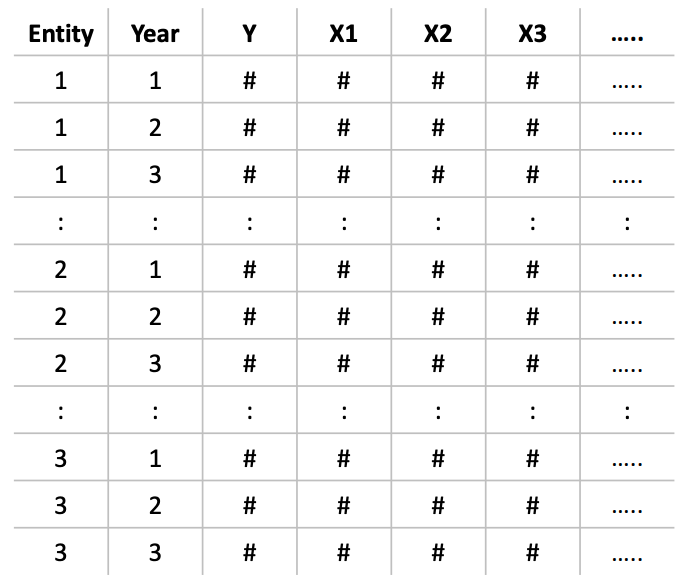
\includegraphics[width=1.2\linewidth]{pictures/PanelData_longform} \end{flushright}
\end{column}
\end{columns}
\end{frame}

\begin{frame}{Panel Data - The Long Form}
\protect\hypertarget{panel-data---the-long-form}{}
\begin{columns}[T]
\begin{column}{.3\textwidth}
\vspace{2cm}

\normalsize

Preparing data into panel data format:

\small
\vspace{2mm}

Entity and Time in rows.

\(\&\)

Variables in columns.
\end{column}

\begin{column}{0.48\textwidth}
\begin{flushright}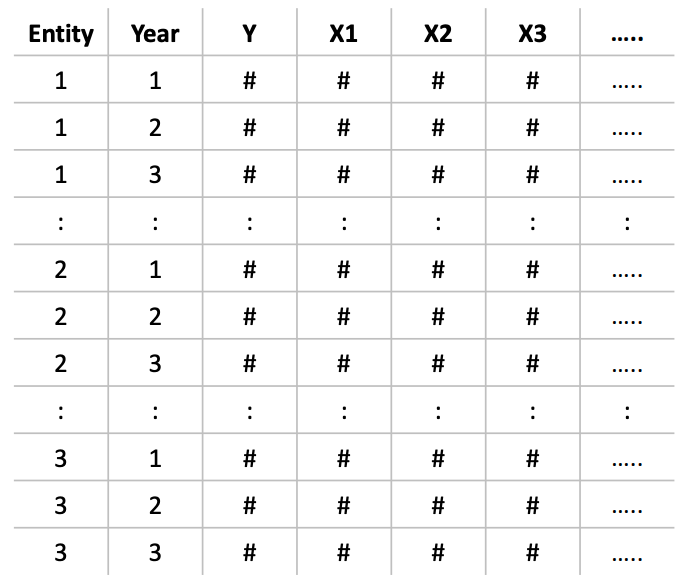
\includegraphics[width=1.2\linewidth]{pictures/PanelData_longform} \end{flushright}
\end{column}
\end{columns}
\end{frame}

\begin{frame}{Balanced Panel}
\protect\hypertarget{balanced-panel}{}
\begin{columns}[T]
\begin{column}{.3\textwidth}
\vspace{2cm}

\small

All entities are observed across all times. \[
\begin{aligned}
\text{51 states} &\times \text{23 years}\\
&\text{= 1173 observations}
\end{aligned}
\]
\end{column}

\begin{column}{0.48\textwidth}
\begin{flushright}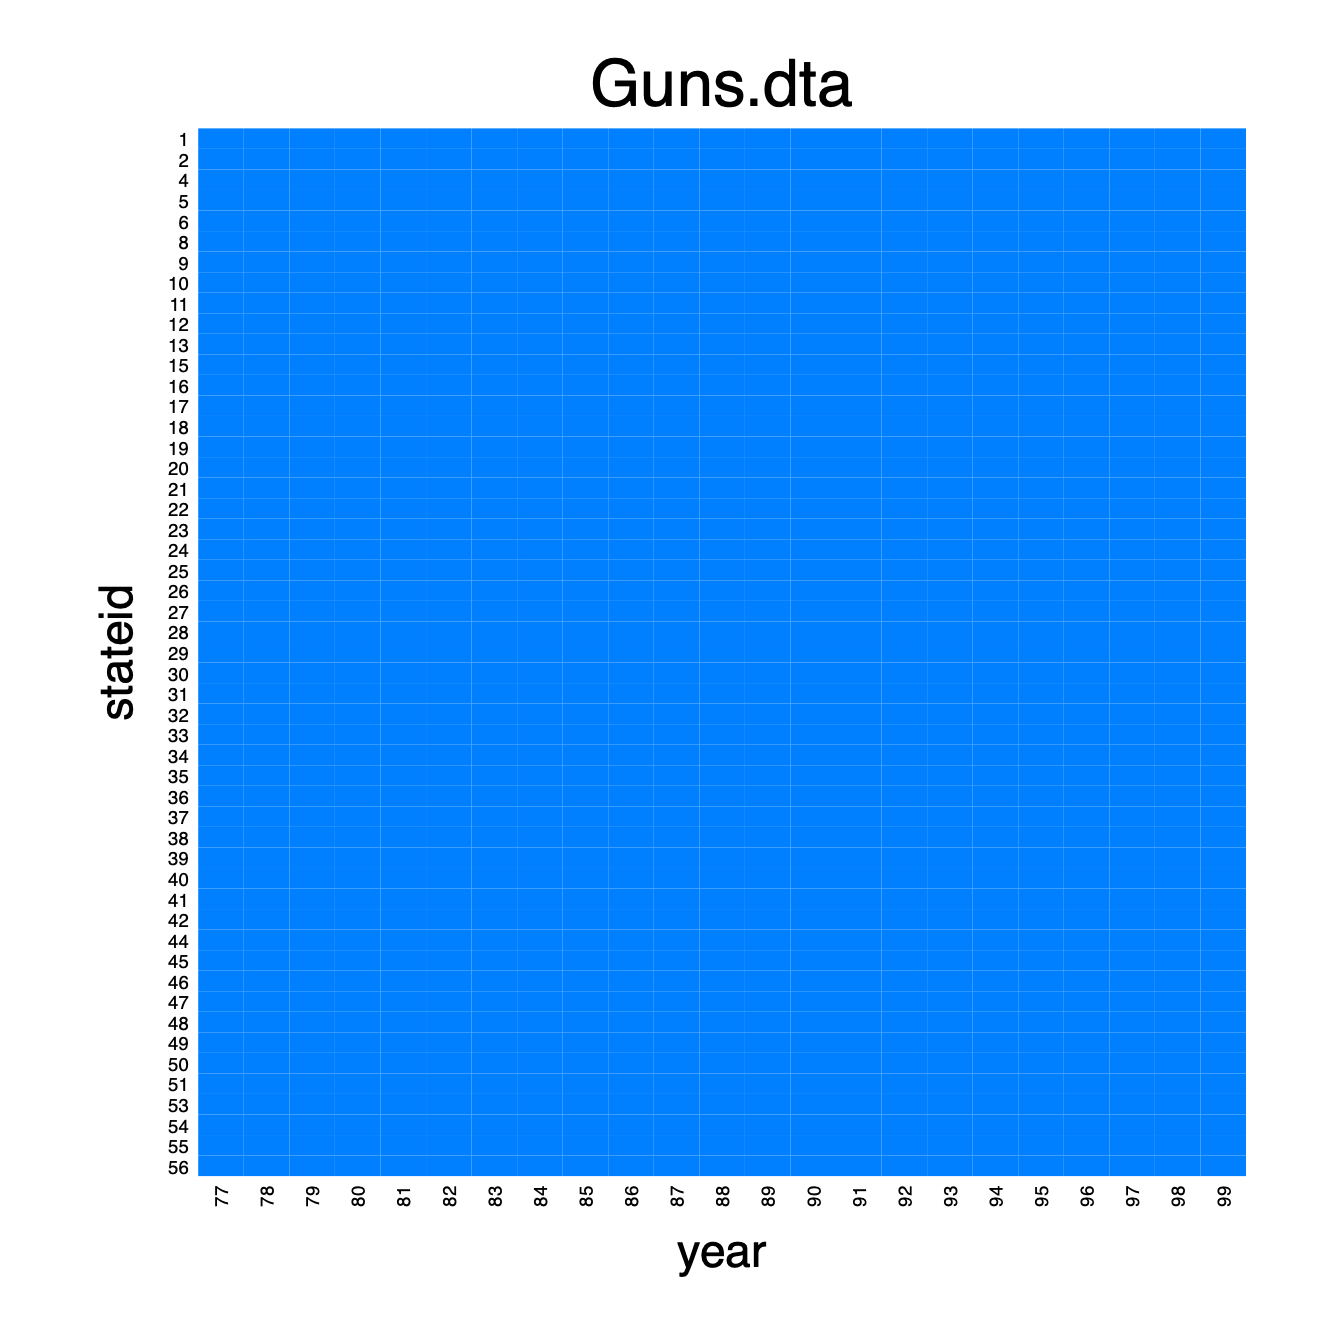
\includegraphics[width=1.25\linewidth]{pictures/Q1-panelView-balanced} \end{flushright}
\end{column}
\end{columns}
\end{frame}

\begin{frame}{Unbalanced Panel}
\protect\hypertarget{unbalanced-panel}{}
\begin{columns}[T]
\begin{column}{.3\textwidth}
\vspace{2cm}

\small

Some entities are not observed in some time periods.
\end{column}

\begin{column}{0.48\textwidth}
\begin{flushright}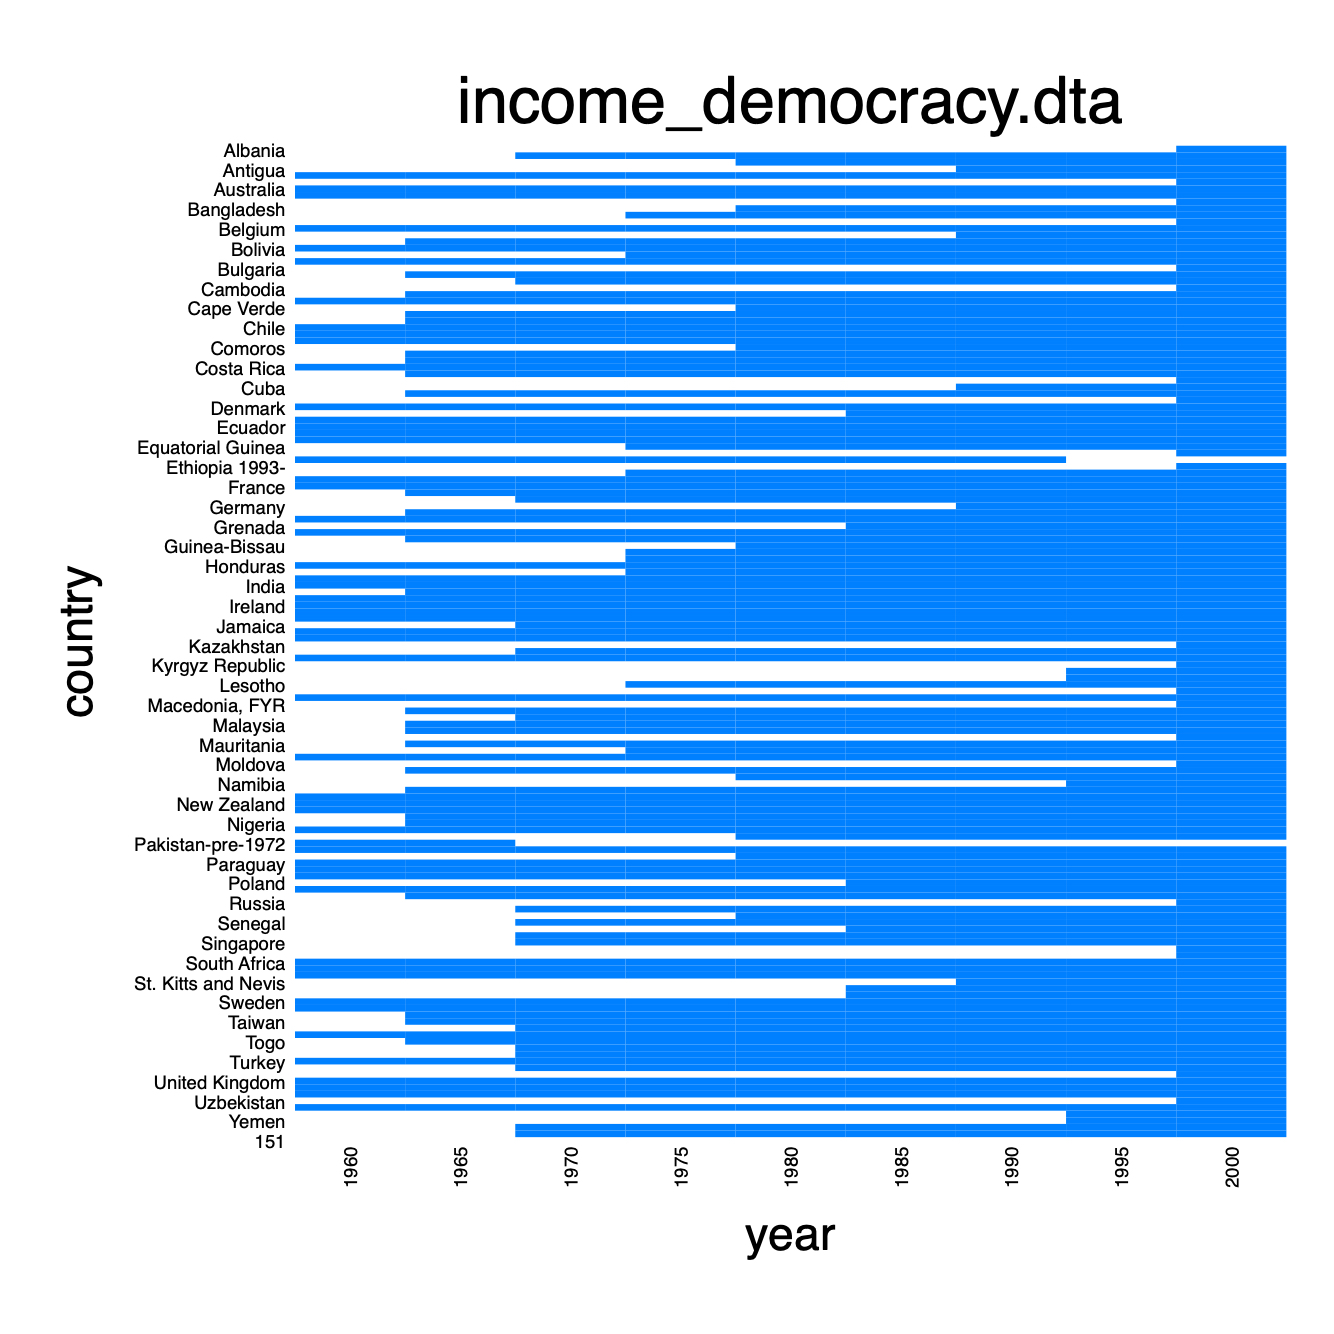
\includegraphics[width=1.25\linewidth]{pictures/Q2-panelView-unbalanced} \end{flushright}
\end{column}
\end{columns}
\end{frame}

\begin{frame}[fragile]{{[}SN{]} STATA command for Setting Data as Panel}
\protect\hypertarget{sn-stata-command-for-setting-data-as-panel}{}
Once the data is in long form, we need to set it as panel so we can use
Stata's panel data \texttt{xt} commands.

\small

\begin{Shaded}
\begin{Highlighting}[]
\NormalTok{*xtset entityid timeid}
\CommentTok{//\textquotesingle{}entityid\textquotesingle{} and \textquotesingle{}timeid\textquotesingle{} have to be in numeric format}
\end{Highlighting}
\end{Shaded}

\begin{center}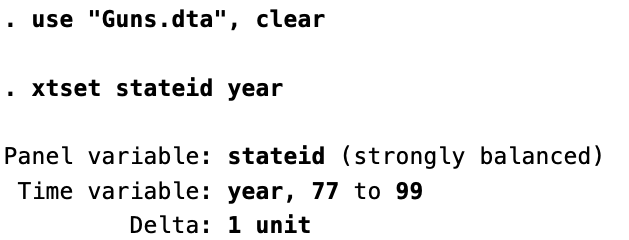
\includegraphics[width=0.48\linewidth]{pictures/Ex1-xtset} 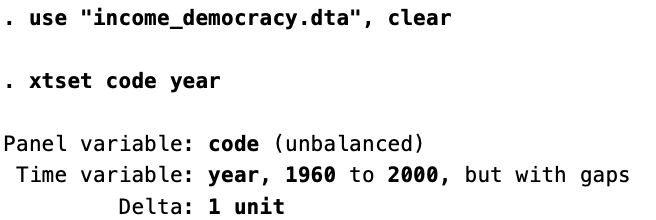
\includegraphics[width=0.48\linewidth]{pictures/Ex2-xtset} \end{center}

\footnotesize

\underline{Note}: \texttt{id} means unique identifiers for entity
(\texttt{entityid}) or for time period (\texttt{timeid})
\end{frame}

\begin{frame}[fragile]{{[}SN{]} STATA command for Visualizing Panel
Data}
\protect\hypertarget{sn-stata-command-for-visualizing-panel-data}{}
Once the data is set as panel, we can use a series of \texttt{xt}
commands to analyze it.

\vspace{3mm}

For visualization \small

\begin{Shaded}
\begin{Highlighting}[]
\NormalTok{*}\KeywordTok{xtline}\NormalTok{ varname\_of\_inteterest}
\CommentTok{//graphs by entities}
\end{Highlighting}
\end{Shaded}

\small

\begin{Shaded}
\begin{Highlighting}[]
\NormalTok{*}\KeywordTok{xtline}\NormalTok{ varname\_of\_inteterest, overlay }\BaseNTok{legend}\NormalTok{(}\KeywordTok{off}\NormalTok{)}
\CommentTok{//all entities in one graph}
\end{Highlighting}
\end{Shaded}
\end{frame}

\begin{frame}{Fixed Effects Regressions - General Form}
\protect\hypertarget{fixed-effects-regressions---general-form}{}
For \(i = 1,\ldots,n\) and \(t = 1,\ldots,T\)

\[
Y_{it} = {\color{gray}{\overbracket{\color{black}{\beta_1 X_{1,it} + \beta_2 X_{2,it} + \ldots + \beta_k X_{k,it}}}^{\text{k regressor}}}} + {\color{red}{\underbracket{\alpha_i}_{\substack{\text{entity}\\ \text{fixed effects}}}}} + {\color{green}{\underbracket{\lambda_t}_{\substack{\text{time}\\ \text{fixed effects}}}}} + u_{it}
\]

\[
\begin{aligned}
&(3) \quad \text{Both E}\&\text{T Fixed Effects: } &Y_{it} &= \beta_1 X_{it} + {\color{red}{\underbracket{\alpha_i}_{\substack{\text{entity}\\ \text{fixed effects}}}}} + {\color{green}{\underbracket{\lambda_t}_{\substack{\text{time}\\ \text{fixed effects}}}}} + u_{it}\\
&(1) \quad \text{Entity Fixed Effects: }
&Y_{it} &= \beta_1 X_{it} + {\color{red}{\alpha_i}} + u_{it}\\
\\
&(2) \quad \text{Time Fixed Effects: }
&Y_{it} &= \beta_1 X_{it} + {\color{green}{\lambda_t}} + u_{it}
\end{aligned}
\]
\end{frame}

\begin{frame}{(1) Entity Fixed Effects (Time-invariant)}
\protect\hypertarget{EntityFEs}{}
\[
Y_{it} =  \beta_1 X_{it} + {\color{red}{\overbracket{\alpha_i}^{\substack{\text{n entity-specific}\\ \text{intercepts}}}}} + u_{it}
\] \[\Downarrow\] \[
Y_{it} = {\color{red}{\underbracket{\beta_0}_{\text{an intercept}}}} + \beta_1 X_{it} + {\color{red}{\underbracket{\gamma_2 D2_i + \gamma_3 D3_i + \ldots + \gamma_n Dn_i}_{\text{with n-1 entity binary indicators}}}} +  u_{it}
\]

Entity \(\mathbf{1}\): \(\alpha_1 = \beta_0\)

Entity \(\mathbf{2}\): \(\alpha_2 = \beta_0 + \gamma_2\)

Entity \(\mathbf{3}\): \(\alpha_3 = \beta_0 + \gamma_3\)

\(\vdots\)

Entity \(\mathbf{n}\): \(\alpha_n = \beta_0 + \gamma_n\)

\footnotesize \underline{Note}: This form suggests estimating regression
model with \(n-1\) binary indicators by OLS, but we can also use
\emph{``entity-demeaned'' OLS algorithm}.
\end{frame}

\begin{frame}{(2) Time Fixed Effects (Entity-invariant)}
\protect\hypertarget{TimeFEs}{}
\[
Y_{it} = \beta_1 X_{it} + {\color{green}{\overbracket{\lambda_t}^{\substack{\text{T time-specific}\\ \text{intercepts}}}}} + u_{it}
\] \[\Downarrow\] \[
Y_{it} = {\color{green}{\underbracket{\beta_0}_{\text{an intercept}}}} + \beta_1 X_{it} + {\color{green}{\underbracket{\delta_2 B2_t + \delta_3 B3_t + \ldots + \delta_T BT_t}_{\text{with n-1 time binary indicators}}}} + u_{it}
\] Time period \(\mathbf{1}\): \(\lambda_1 = \beta_0\)

Time period \(\mathbf{2}\): \(\lambda_2 = \beta_0 + \delta_2\)

Time period \(\mathbf{3}\): \(\lambda_3 = \beta_0 + \delta_3\)

\(\vdots\)

Time period \(\mathbf{T}\): \(\lambda_T = \beta_0 + \delta_T\)

\footnotesize \underline{Note}: This form suggests estimating regression
model with \(T-1\) binary indicators by OLS, but we can also use
\emph{``time-demeaned'' OLS algorithm}.
\end{frame}

\begin{frame}{(3) Both Entity and Time (Two-way) Fixed Effects}
\protect\hypertarget{BothFEs}{}
\[
Y_{it} = \beta_1 X_{it} + {\color{red}{\overbracket{\alpha_i}^{\substack{\text{entity}\\ \text{fixed effects}}}}} + {\color{green}{\overbracket{\lambda_t}^{\substack{\text{time}\\ \text{fixed effects}}}}} + u_{it}
\] \[\Downarrow\] \[
\begin{aligned}
Y_{it} = {\color{blue}{\underbracket{\beta_0}_{\text{an intercept}}}} + \beta_1 X_{it} 
&+ {\color{red}{\underbracket{\gamma_2 D2_i + \gamma_3 D3_i + \ldots + \gamma_n Dn_i}_{\text{with n-1 entity binary indicators}}}} \\
&+ {\color{green}{\underbracket{\delta_2 B2_t + \delta_3 B3_t + \ldots + \delta_T BT_t}_{\text{with n-1 time binary indicators}}}}
+  u_{it}
\end{aligned}
\]

\vspace{3mm}

\footnotesize \underline{Note}: This form suggests estimating regression
model with \(n-1\) entity binary indicators and \(T-1\) time binary
indicators by OLS, but we can also combine with \emph{``demeaned'' OLS
algorithm}.
\end{frame}

\begin{frame}[fragile]{{[}SN{]} STATA syntax for Fixed Effects
Regressions}
\protect\hypertarget{sn-stata-syntax-for-fixed-effects-regressions}{}
\normalsize(1) \textcolor{red}{Entity} Fixed Effects\small

\begin{Shaded}
\begin{Highlighting}[]
\NormalTok{*}\KeywordTok{xtreg}\NormalTok{ yvar xvar, }\KeywordTok{fe} \KeywordTok{vce}\NormalTok{(}\KeywordTok{cluster}\NormalTok{ entityid)}
\end{Highlighting}
\end{Shaded}

\normalsize(2) \textcolor{green}{Time} Fixed Effects\small

\begin{Shaded}
\begin{Highlighting}[]
\NormalTok{*}\KeywordTok{regress}\NormalTok{ yvar xvar i.timeid, }\KeywordTok{fe} \KeywordTok{vce}\NormalTok{(}\KeywordTok{cluster}\NormalTok{ entityid)}
\end{Highlighting}
\end{Shaded}

\normalsize(3) Both \textcolor{red}{Entity} \(\&\)
\textcolor{green}{Time} Fixed Effects\small

\begin{Shaded}
\begin{Highlighting}[]
\NormalTok{*}\KeywordTok{xtreg}\NormalTok{ yvar xvar i.timeid, }\KeywordTok{fe} \KeywordTok{vce}\NormalTok{(}\KeywordTok{cluster}\NormalTok{ entityid)}
\end{Highlighting}
\end{Shaded}

\footnotesize

\underline{Note}: \texttt{id} means unique identifiers for entity
(\texttt{entityid}) or for time period (\texttt{timeid})
\end{frame}

\begin{frame}[fragile]{Clustered Standard Errors}
\protect\hypertarget{ClusteredSE}{}
\[
\begin{matrix}
    & {\color{green}{t=1}}     & {\color{green}{t=2}}    & \ldots & {\color{green}{t=T}}
\\
{\color{red}{i=1}} & u_{11}  & u_{12} & \ldots & u_{1T}
\\
{\color{red}{i=2}} & u_{21}  & u_{22} & \ldots & u_{2T}
\\
\vdots & \vdots & \vdots & \ldots & \vdots
\\
{\color{red}{i=n}} & u_{n1}  & u_{n2} & \ldots & u_{nT}
\\
\end{matrix}
\]

\begin{itemize}
\item
  Sampling are \textcolor{red}{\textit{i.i.d}} across entities.
\item
  But if the omitted factors comprising the error term \(u_{it}\) are
  serially correlated, then \(u_{it}\) is serially correlated aka
  \textcolor{green}{\textit{autocorrelated}} - that is, correlated over
  time within an entity.
\end{itemize}

Standard errors need to allow both for this autocorrelation and for
potential heteroskedasticity \(\rightarrow\) use \textbf{clustered
standard errors}.

\small

\begin{Shaded}
\begin{Highlighting}[]
\NormalTok{*[, }\KeywordTok{vce}\NormalTok{(}\KeywordTok{cluster}\NormalTok{ entityid)]}
\CommentTok{//add this option at the end of STATA regressions }
\end{Highlighting}
\end{Shaded}
\end{frame}

\hypertarget{excercise-1-based-on-stock-watson-e10.1}{%
\section{Excercise 1: based on Stock \& Watson,
E10.1}\label{excercise-1-based-on-stock-watson-e10.1}}

\begin{frame}[fragile]{Excercise 1: based on Stock \& Watson, E10.1}
\begin{itemize}
\tightlist
\item
  \textbf{Objective:} Analyze effects of \emph{concealed weapons laws}
  on \emph{violent crimes}.

  \begin{itemize}
  \tightlist
  \item
    {[}Proponents:{]} More people carry concealed weapons, crime will
    decline because criminals will be deterred from attacking other
    people.
  \item
    {[}Opponents:{]} Crime will increase because of accidental or
    spontaneous use of the weapons.
  \end{itemize}
\end{itemize}

\vspace{0.8mm}

\begin{itemize}
\tightlist
\item
  \textbf{Dataset:} \texttt{Guns.dta}

  \begin{itemize}
  \tightlist
  \item
    A balanced panel of data from the 50 U.S. states plus the District
    of Columbia for 23 years (1977-1999).
  \end{itemize}
\end{itemize}

\vspace{0.8mm}

\begin{itemize}
\tightlist
\item
  \textbf{Key variables:}

  \begin{itemize}
  \tightlist
  \item
    \texttt{stateid}: ID number of states (Alabama = 1, Alaska = 2,
    etc.)
  \item
    \texttt{year}: year (1977-1999)
  \item
    \texttt{shall}: \(=1\) if the state has a shall-carry law in effect
    in that year \(=0\) otherwise
  \item
    \texttt{vio}: violent crime rate.
  \end{itemize}
\end{itemize}
\end{frame}

\begin{frame}{Variable Description}
\protect\hypertarget{variable-description}{}
\begin{center}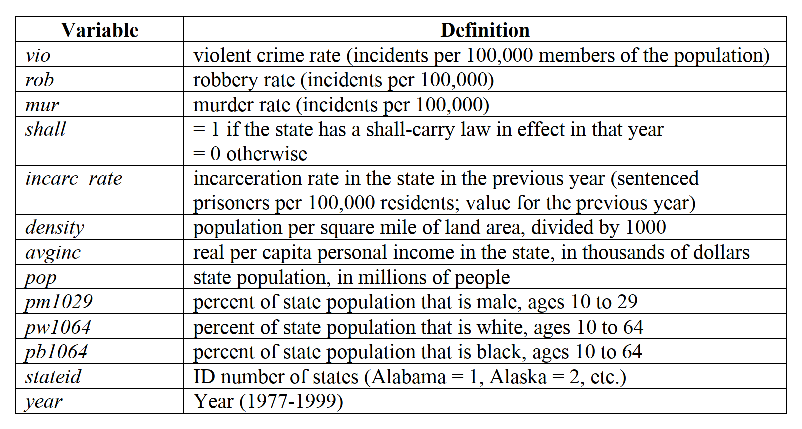
\includegraphics[width=0.95\linewidth]{pictures/Ex1-VarDef} \end{center}
\footnotesize

Source:
\href{https://ianayres.yale.edu/sites/default/files/files/Ayres_Donohue_article.pdf}{Ayres,
I. and Donohue, J.J., 2002. Shooting down the more guns, less crime
hypothesis.}
\end{frame}

\begin{frame}{}
\protect\hypertarget{section}{}
\begin{center}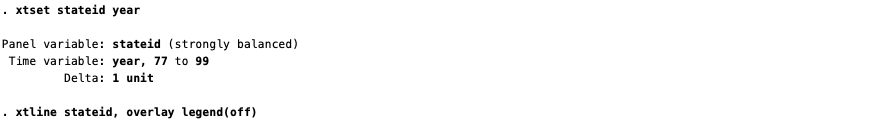
\includegraphics[width=1\linewidth]{pictures/Ex1-xtset-xtline} \end{center}

\begin{center}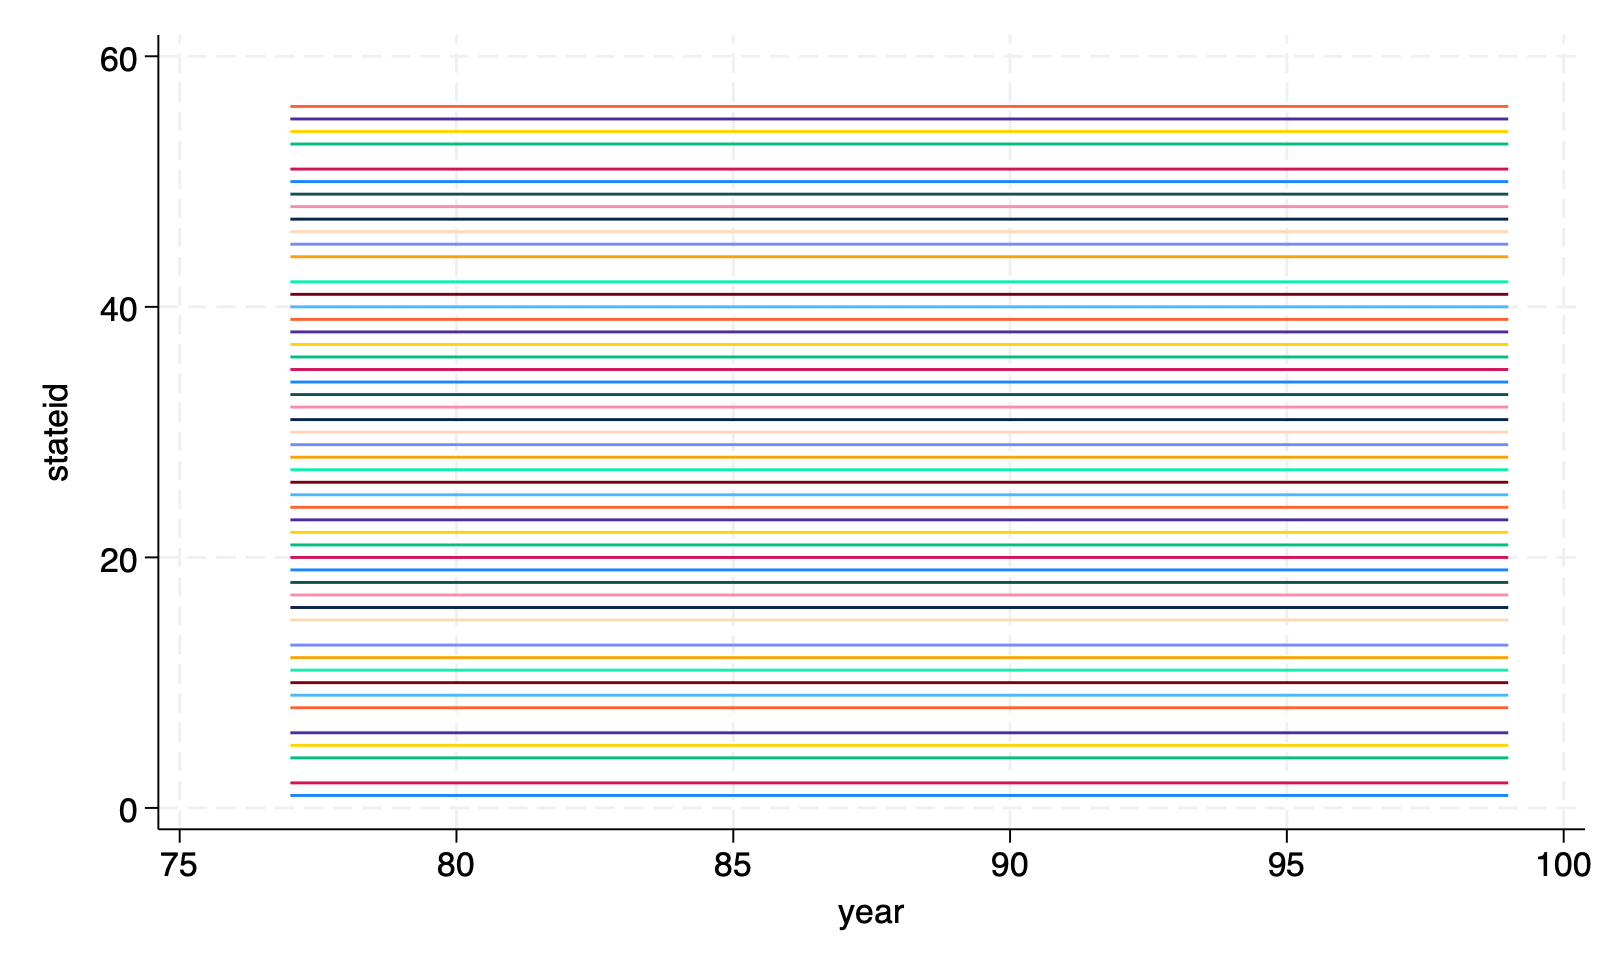
\includegraphics[width=1\linewidth]{pictures/Q1-panelView} \end{center}
\end{frame}

\begin{frame}[fragile]{Questions}
\protect\hypertarget{questions}{}
\begin{enumerate}
[(a)]
\tightlist
\item
  Estimate a linear regression model of:
\end{enumerate}

\begin{itemize}
\item
  (M1) \texttt{ln(vio)} against \texttt{shall}.
\item
  (M2) \texttt{ln(vio)} against \texttt{shall}, \texttt{incarc\_rate},
  \texttt{density}, \texttt{avginc}, \texttt{pop}, \texttt{pb1064},
  \texttt{pw1064} and \texttt{pm1029}.
\end{itemize}

\begin{enumerate}
[i.]
\item
  Interpret the coefficient on shall in (M2).\\
  Is this estimate large or small in a real-world sense?
\item
  Does adding the control variables in (M2) change the estimated effect
  of a shall-issue law in (M1) as measured by statistical significance?
  As measured by the real-world significance of the estimated
  coefficient?
\item
  Suggest a variable that varies across states but plausibly varies
  little or not at all over time and that could cause omitted variable
  bias in (M2).
\end{enumerate}
\end{frame}

\begin{frame}[fragile]{Questions}
\protect\hypertarget{questions-1}{}
\begin{enumerate}
[(a)]
\setcounter{enumi}{1}
\tightlist
\item
  Do the results change when you add \emph{state fixed effects}?\\
  If so, which set of regression results is more credible, and why?
\end{enumerate}

\vspace{3mm}

\begin{enumerate}
[(a)]
\setcounter{enumi}{2}
\tightlist
\item
  Do the results change when you add \emph{time fixed effects}?\\
  If so, which set of regression results is more credible, and why?
\end{enumerate}

\vspace{3mm}

\begin{enumerate}
[(a)]
\setcounter{enumi}{3}
\tightlist
\item
  Repeat the analysis using \texttt{ln(rob)} and \texttt{ln(mur)} in
  place of \texttt{ln(vio)}.
\end{enumerate}
\end{frame}

\begin{frame}{(a-i,ii) Estimate linear regression models (M1) and (M2)}
\protect\hypertarget{Ex1-pooledOLS-A}{}
From OLS estimation results for (M1)
\footnotesize \protect\hyperlink{Ex1-pooledsimple}{(\textgreater\textgreater stata)}
\normalsize and (M2)
\footnotesize \protect\hyperlink{Ex1-pooledwithctrls}{(\textgreater\textgreater stata)}
\normalsize

\begin{itemize}
\item
  The coefficient is \(-0.368\), which suggests that shall-issue laws
  reduce violent crime by \(36\%\). This is a large effect.
\item
  The coefficient in (1) is \(-0.443\); in (2) it is \(-0.368\). Both
  are highly statistically significant. Adding the control variables
  results in a small drop in the coefficient.
\end{itemize}
\end{frame}

\begin{frame}[fragile]{(a-iii) Suggest a variable that varies across
states but plausibly varies little or not at all over time and that
could cause omitted variable bias in (M2).}
\protect\hypertarget{a-iii-suggest-a-variable-that-varies-across-states-but-plausibly-varies-little-or-not-at-all-over-time-and-that-could-cause-omitted-variable-bias-in-m2.}{}
There are several examples:

\begin{itemize}
\item
  Residents' attitudes towards guns and crime, these are typically slow
  to change.
\item
  Quality of police and other crime-prevention programs.
\item
  For historical reasons, cities can have very different crime rates.
\item
  Geographic features.
\item
  etc.
\end{itemize}

\(\Longrightarrow\) These factors constitute an \emph{unobserved state
effect}/ \emph{state fixed effect}/ \emph{unobserved state
heterogeneity}. If they and the variable of interest (\texttt{shall})
are correlated, omitting such variables results in OVB
(\textbf{heterogeneity bias}).
\end{frame}

\begin{frame}{(b) Do the results change when you add \emph{state fixed
effects}?}
\protect\hypertarget{b-do-the-results-change-when-you-add-state-fixed-effects}{}
Good news: These time-invariant factors can be effectively captured by
the state fixed effect \(\alpha_i\)!
\footnotesize \protect\hyperlink{EntityFEs}{(\textgreater\textgreater review)}
\normalsize
\end{frame}

\begin{frame}[fragile]{(b) Do the results change when you add
\emph{state fixed effects}?}
\protect\hypertarget{b-do-the-results-change-when-you-add-state-fixed-effects-1}{}
\footnotesize

\begin{Shaded}
\begin{Highlighting}[]
\NormalTok{*}\KeywordTok{xtreg}\NormalTok{ yvar xvar, }\KeywordTok{fe} \KeywordTok{vce}\NormalTok{(}\KeywordTok{cluster}\NormalTok{ entityid)}
\end{Highlighting}
\end{Shaded}

\begin{flushleft}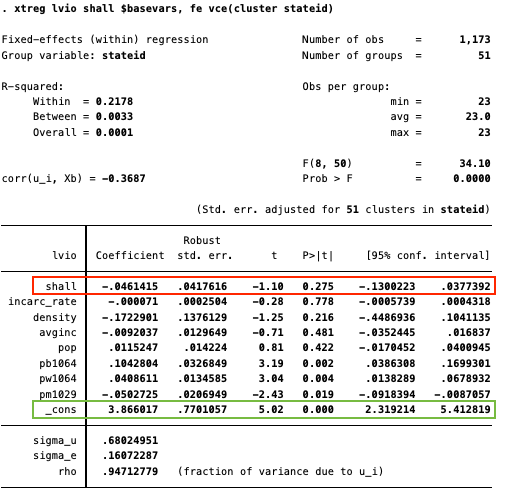
\includegraphics[width=0.8\linewidth]{pictures/Ex1-EntityFEs} \end{flushleft}
\end{frame}

\begin{frame}[fragile]{(b) Do the results change when you add
\emph{state fixed effects}?}
\protect\hypertarget{b-do-the-results-change-when-you-add-state-fixed-effects-2}{}
\begin{itemize}
\item
  In (M3) the coefficient on shall falls to \(-0.046\), a large
  reduction in the coefficient from (M2). The estimate is not
  statistically significantly different from zero.
\item
  Evidently there was important omitted variable bias leading to a
  spurious effect in (M2).
\item
  The constant reported in \texttt{xtreg,\ fe} results implies the
  estimated average fixed effect.
\end{itemize}

\vspace{2mm}

\small \textcolor{gray}{Like experiments $\rightarrow$ Let's compare:}

\footnotesize

\begin{Shaded}
\begin{Highlighting}[]
\KeywordTok{reg}\NormalTok{ lvio shall i.stateid }
\end{Highlighting}
\end{Shaded}

\begin{Shaded}
\begin{Highlighting}[]
\KeywordTok{xtreg}\NormalTok{ lvio shall, }\KeywordTok{fe}
\end{Highlighting}
\end{Shaded}
\end{frame}

\begin{frame}[fragile]{(c) Do the results change when you add \emph{time
fixed effects}?}
\protect\hypertarget{c-do-the-results-change-when-you-add-time-fixed-effects}{}
\footnotesize

\begin{Shaded}
\begin{Highlighting}[]
\NormalTok{*}\KeywordTok{xtreg}\NormalTok{ yvar xvar i.timeid, }\KeywordTok{fe} \KeywordTok{vce}\NormalTok{(}\KeywordTok{cluster}\NormalTok{ entityid)}
\end{Highlighting}
\end{Shaded}

\begin{flushleft}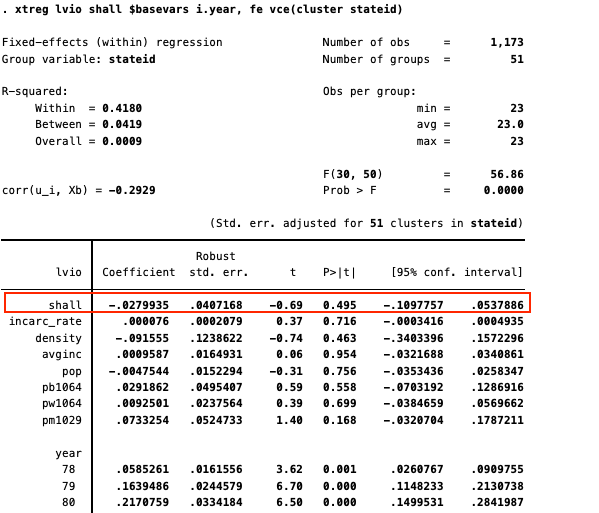
\includegraphics[width=0.8\linewidth]{pictures/Ex1-TwowayFEs-5} \end{flushleft}
\end{frame}

\begin{frame}{(c) Do the results change when you add \emph{time fixed
effects}?}
\protect\hypertarget{c-do-the-results-change-when-you-add-time-fixed-effects-1}{}
\begin{flushleft}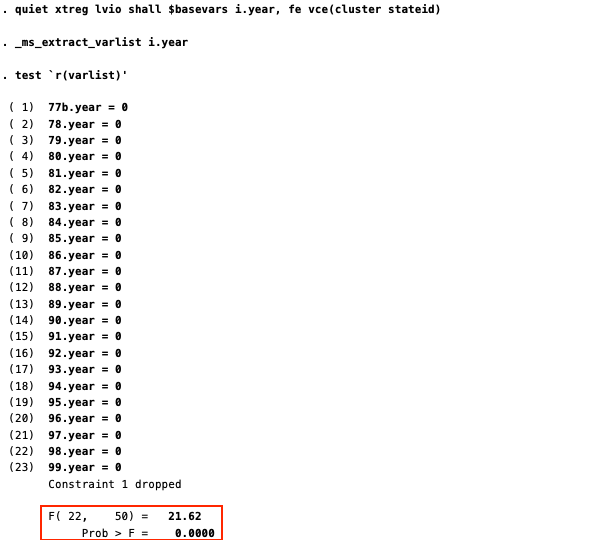
\includegraphics[width=0.7\linewidth]{pictures/Ex1-TestTimeFEs-2} \end{flushleft}
\end{frame}

\begin{frame}{(c) Do the results change when you add \emph{time fixed
effects}?}
\protect\hypertarget{c-do-the-results-change-when-you-add-time-fixed-effects-2}{}
\begin{itemize}
\item
  The coefficient falls further to \(-0.028\). The coefficient is
  insignificantly different from zero.
\item
  The time effects are jointly statistically significant, so this
  regression seems better specified than (M3).
\end{itemize}
\end{frame}

\begin{frame}{Table of Results - Exercise 1}
\protect\hypertarget{table-of-results---exercise-1}{}
\small
\begin{table}[]
\centering
\begin{tabular}{|l|cccc|}
\hline
\multicolumn{1}{|c|}{\multirow{2}{*}{\textbf{Regressor}}} &
  \multicolumn{4}{c|}{\textbf{Models}} \\ \cline{2-5}
\multicolumn{1}{|c|}{} &
  \multicolumn{1}{c|}{\textbf{(M1)}} &
  \multicolumn{1}{c|}{\textbf{(M2)}} &
  \multicolumn{1}{c|}{\textbf{(M3)}} &
  \textbf{(M4)} \\ \hline
\textit{shall} &
  \multicolumn{1}{c|}{\begin{tabular}[c]{@{}c@{}}{\color{red}{-0.443***}}\\ (0.157)\\ {[}-0.76, -0.13{]}\end{tabular}} &
  \multicolumn{1}{c|}{\begin{tabular}[c]{@{}c@{}}{\color{red}{-0.368***}}\\ (0.114)\\ {[}-0.60, -0.14{]}\end{tabular}} &
  \multicolumn{1}{c|}{\begin{tabular}[c]{@{}c@{}}{\color{red}{-0.0461}}\\ (0.042)\\ {[}-0.13, 0.04{]}\end{tabular}} &
  \begin{tabular}[c]{@{}c@{}}{\color{red}{-0.0280}}\\ (0.041)\\ {[}-0.11, 0.05{]}\end{tabular} \\ \hline
\textit{Controls} &
  \multicolumn{1}{c|}{No} &
  \multicolumn{1}{c|}{Yes} &
  \multicolumn{1}{c|}{Yes} &
  Yes \\ \hline
\textit{State effects} &
  \multicolumn{1}{c|}{No} &
  \multicolumn{1}{c|}{No} &
  \multicolumn{1}{c|}{Yes} &
  Yes \\ \hline
\textit{Time effects} &
  \multicolumn{1}{c|}{No} &
  \multicolumn{1}{c|}{No} &
  \multicolumn{1}{c|}{No} &
  Yes \\ \hline
\end{tabular}
\end{table}
\footnotesize

Notes: Clustered standard errors shown in parentheses and \(95\%\)
confidence intervals are shown in brackets;
\(\text{***} p<0.01\),\(\text{**} p<0.05\),\(\text{*} p<0.1\).
\end{frame}

\hypertarget{excercise-2-based-on-stock-watson-e10.2}{%
\section{Excercise 2: based on Stock \& Watson,
E10.2}\label{excercise-2-based-on-stock-watson-e10.2}}

\begin{frame}[fragile]{Picture the Scenario}
\protect\hypertarget{picture-the-scenario}{}
\begin{itemize}
\tightlist
\item
  \textbf{Objective:} Do citizens demand more democracy and political
  freedom as their incomes grow? That is, is democracy a normal good?
\end{itemize}

\vspace{0.8mm}

\begin{itemize}
\tightlist
\item
  \textbf{Dataset:} \texttt{Income-Democracy.dta}

  \begin{itemize}
  \tightlist
  \item
    a panel data set from \(195\) countries for the years
    \(1960, 1965,\ldots,2000\).
  \end{itemize}
\end{itemize}

\vspace{0.8mm}

\begin{itemize}
\tightlist
\item
  \textbf{Key variables:} For each country in each year

  \begin{itemize}
  \tightlist
  \item
    \texttt{Dem\_ind}: an index of political freedom/democracy.
  \item
    \texttt{Log\_GDPPC}: per capita income.
  \item
    various demographic controls.
  \end{itemize}
\end{itemize}
\end{frame}

\begin{frame}{Variable Description}
\protect\hypertarget{variable-description-1}{}
\begin{center}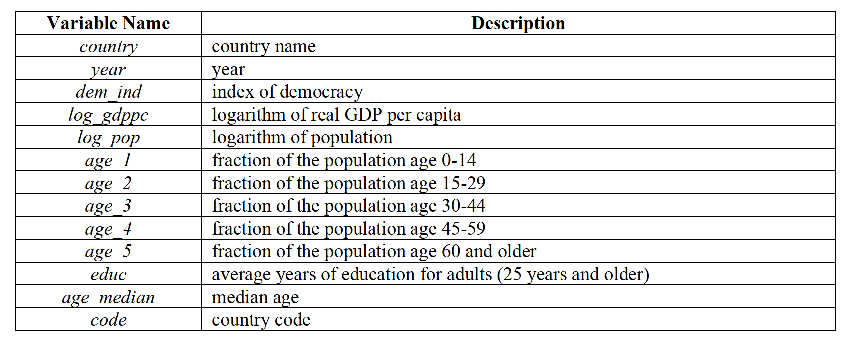
\includegraphics[width=1\linewidth]{pictures/Ex2-VarDef} \end{center}
\footnotesize

Source:
\href{https://www.aeaweb.org/articles?id=10.1257/aer.98.3.808}{Acemoglu,
Daron, Simon Johnson, James A. Robinson, and Pierre Yared. 2008.
``Income and Democracy.'' American Economic Review, 98 (3): 808-42.}

Notes: The income and demographic variable are lagged five years.
\end{frame}

\begin{frame}{}
\protect\hypertarget{section-1}{}
\begin{center}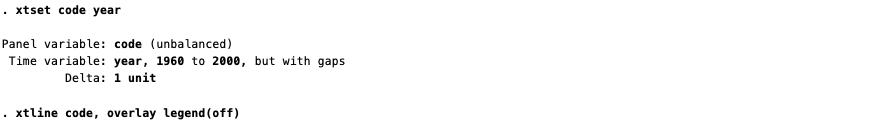
\includegraphics[width=1\linewidth]{pictures/Ex2-xtset-xtline} \end{center}

\begin{center}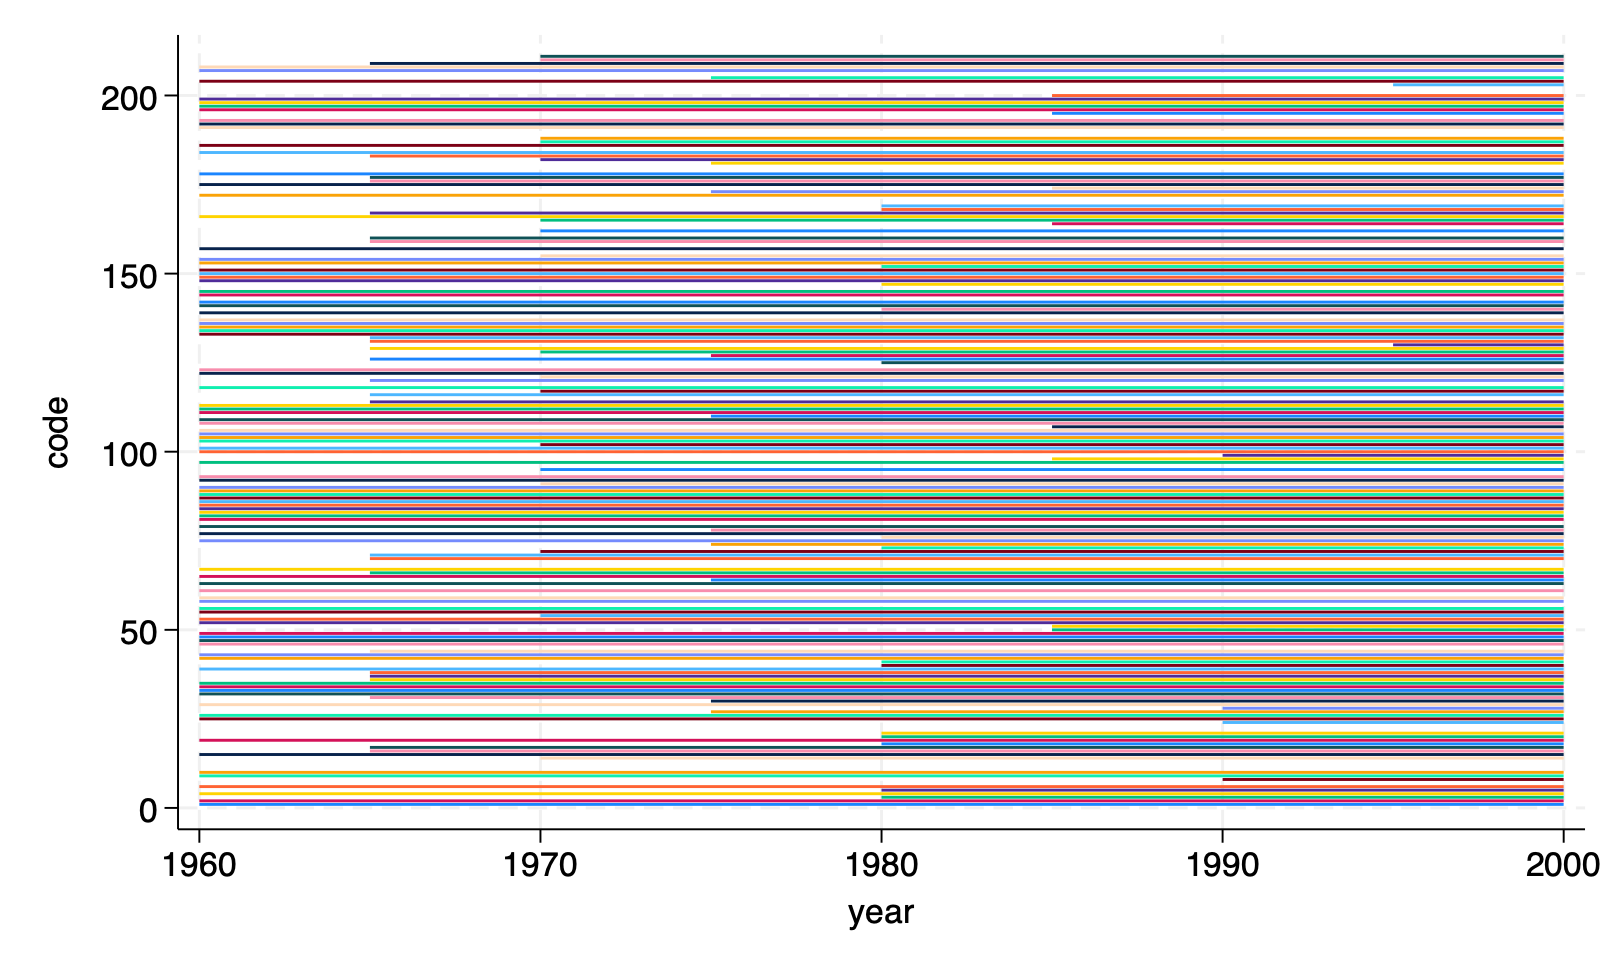
\includegraphics[width=1\linewidth]{pictures/Q2-panelView} \end{center}
\end{frame}

\begin{frame}[fragile]{Questions}
\protect\hypertarget{questions-2}{}
\begin{enumerate}
[(a)]
\tightlist
\item
  Is the data set a balanced panel? Explain.
\end{enumerate}

\vspace{3mm}

\begin{enumerate}
[(a)]
\setcounter{enumi}{1}
\tightlist
\item
  The logarithm of per capita income is labeled \texttt{Log\_GDPPC}.
  Regress \texttt{Dem\_ind} on \texttt{Log\_GDPPC}. Use standard errors
  that are clustered by country.
\end{enumerate}

\begin{enumerate}
[i.]
\item
  How large is the estimated coefficient on \texttt{Log\_GDPPC}?\\
  Is the coefficient statistically significant?
\item
  If per capita income in a country increases by \(20\%\), by how much
  is \texttt{Dem\_ind} predicted to increase?\\
  What is a \(95\%\) confidence interval for the prediction?\\
  Is the predicted increase in \texttt{Dem\_ind} large or small?
  (Explain what you mean by large or small.)
\item
  Why is it important to use clustered standard errors for the
  regression?\\
  Do the results change if you do not use clustered standard errors?
\end{enumerate}
\end{frame}

\begin{frame}{Questions}
\protect\hypertarget{questions-3}{}
\begin{enumerate}
[(a)]
\setcounter{enumi}{2}
\tightlist
\item
  Estimate the regression in (b), allowing for country fixed effects.
  How do your answers to (b-i) change?
\end{enumerate}

\vspace{3mm}

\begin{enumerate}
[(a)]
\setcounter{enumi}{3}
\tightlist
\item
  Estimate the regression in (b), allowing for time and country fixed
  effects. How do your answers to (b-i) change?
\end{enumerate}

\vspace{3mm}

\begin{enumerate}
[(a)]
\setcounter{enumi}{4}
\tightlist
\item
  There are additional demographic controls in the data set. Should
  these variables be included in the regression? If so, how do the
  results change when they are included?
\end{enumerate}
\end{frame}

\begin{frame}[fragile]{(a) Is the data set a balanced panel? Explain.}
\protect\hypertarget{a-is-the-data-set-a-balanced-panel-explain.}{}
\begin{itemize}
\tightlist
\item
  The dataset is unbalanced because data are available over different
  years for different countries. For example, data on \texttt{Dem\_ind}
  are available \vspace{0.8mm}

  \begin{itemize}
  \tightlist
  \item
    for Andorra during 1970, 1995, and 2000;
  \item
    for Afghanistan during \(1960, 1965, \ldots, 2000\).
  \end{itemize}
\end{itemize}
\end{frame}

\begin{frame}{(b) Regress \texttt{Dem\_ind} on \texttt{Log\_GDPPC} using
standard errors clustered by country.}
\protect\hypertarget{b-regress-dem_ind-on-log_gdppc-using-standard-errors-clustered-by-country.}{}
\begin{flushleft}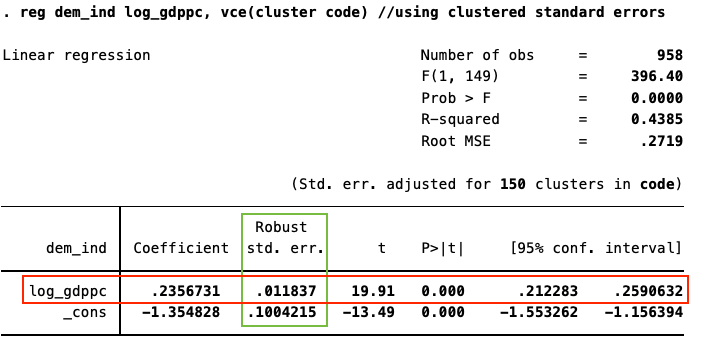
\includegraphics[width=0.9\linewidth]{pictures/Ex2-pooledsimplewithclustering} \end{flushleft}
\end{frame}

\begin{frame}{(b-i) How large is the estimated coefficient on
\texttt{Log\_GDPPC}?}
\protect\hypertarget{b-i-how-large-is-the-estimated-coefficient-on-log_gdppc}{}
\[
\underset{(clustered \enspace se)}{\reallywidehat{Dem\_ind}} = \underset{(.100)}{-1.35} +  \underset{(.012)}{.236} \cdot Log\_GDPPC 
\]

The coefficient is \(0.236\) with a standard error of \(0.012\). The
\(95\%\) confidence interval is \(0.212\) to \(0.259\). The coefficient
is statistically significant.
\end{frame}

\begin{frame}[fragile]{(b-ii) If per capita income in a country
increases by \(20\%\), by how much is \texttt{Dem\_ind} predicted to
increase?}
\protect\hypertarget{b-ii-if-per-capita-income-in-a-country-increases-by-20-by-how-much-is-dem_ind-predicted-to-increase}{}
\footnotesize \textcolor{gray}{Hint: Review Regression models with functional forms involving logarithms; $20\%$ is a big leap for approximation though.}
\normalsize

\vspace{0.8mm}

\begin{itemize}
\tightlist
\item
  A \(20\%\) increase in GDP per capita implies that \texttt{Log\_GDPPC}
  increases by approximately \(0.20\), so that \texttt{Dem\_ind} is
  predicted to increase by approximately \(0.20\times0.236 = 0.0472\),
  or about \(1/8\) of the standard deviation in the dataset.
\end{itemize}

\vspace{0.8mm}

\begin{itemize}
\tightlist
\item
  The \(95\%\) confidence for the effect is (approximately)
  \(0.20\times0.212\) to \(0.20\times0.259 = 0.0472\) or \(0.0424\) to
  \(0.0518\).
\end{itemize}
\end{frame}

\begin{frame}{(b-iii) Why is it important to use clustered standard
errors \quad for the regression?}
\protect\hypertarget{b-iii-why-is-it-important-to-use-clustered-standard-errors-for-the-regression}{}
Compare two models with vs without clustered standard errors
\footnotesize \protect\hyperlink{ClusteredSE}{(\textgreater\textgreater review)}
\normalsize

\begin{center}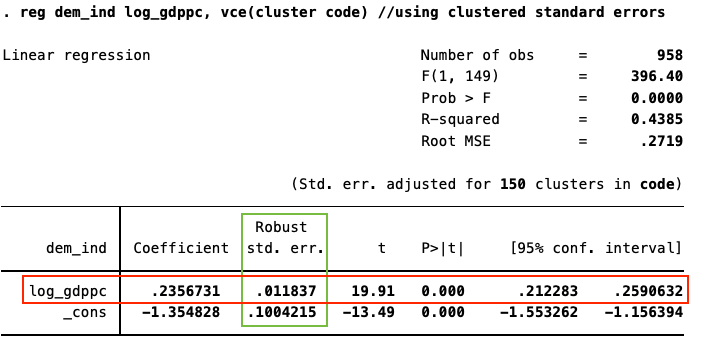
\includegraphics[width=0.49\linewidth]{pictures/Ex2-pooledsimplewithclustering} 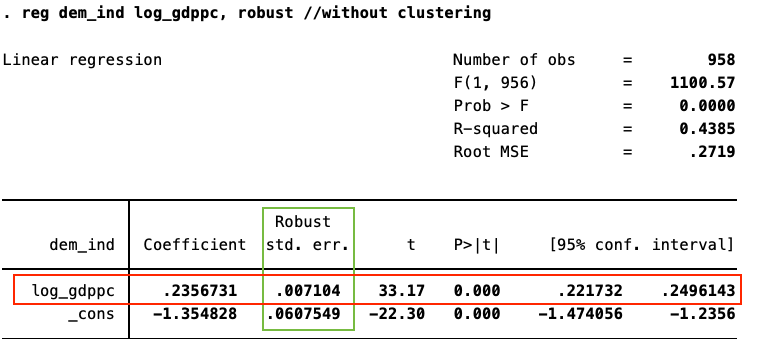
\includegraphics[width=0.49\linewidth]{pictures/Ex2-pooledsimplemoclustering} \end{center}
\end{frame}

\begin{frame}[fragile]{(b-iii) Why is it important to use clustered
standard errors \quad for the regression?}
\protect\hypertarget{b-iii-why-is-it-important-to-use-clustered-standard-errors-for-the-regression-1}{}
\begin{itemize}
\tightlist
\item
  Clustered standard errors are needed because of country-specific
  omitted factors in the regressions.
\end{itemize}

\vspace{0.8mm}

\begin{itemize}
\tightlist
\item
  The clustered standard error for \texttt{Dem\_ind} is \(0.012\); the
  unclustered standard error is smaller (\(0.007\)) because it ignores
  the positive within-country autocorrelation of the errors.
\end{itemize}
\end{frame}

\begin{frame}{(c) Estimate the regression in (b), allowing for country
fixed effects.}
\protect\hypertarget{Ex2-CountryFEs-A}{}
Estimation result
\footnotesize \protect\hyperlink{Ex2-CountryFEs}{(\textgreater\textgreater stata)}
\normalsize

The estimated coefficient falls by a factor of \(3\), to \(0.083\) with
a standard error of \(0.032\). The estimated effect, while significantly
smaller is still statistically significant at the \(1\%\) significance
level.
\end{frame}

\begin{frame}{(d) Estimate the regression in (b), allowing for time and
country fixed effects.}
\protect\hypertarget{Ex2-BothFEs-A}{}
Estimation and test results
\footnotesize \protect\hyperlink{Ex2-BothFEs}{(\textgreater\textgreater stata)}
\normalsize

The estimated coefficient falls further to \(0.054\), approximately
\(1/5\) of the value that omits time and country fixed effects. The
estimate is not statistically significant at the \(10\%\) level.
\end{frame}

\begin{frame}[fragile]{(e) Include additional demographic controls in
the regression.}
\protect\hypertarget{Ex2-BothFEswithcontrols-A}{}
Estimation and test results
\footnotesize \protect\hyperlink{Ex2-BothFEswithcontrols}{(\textgreater\textgreater stata)}
\normalsize

When age, population, and education are included, the estimated
coefficient on \texttt{Log\_GDPPC} falls further to \(0.025\) with a
standard error of \(0.054\). Jointly, these variables are not
statistically significant in the regression, although the age variables
are significant at the \(10\%\) level.
\end{frame}

\begin{frame}{Table of Results - Exercise 2}
\protect\hypertarget{table-of-results---exercise-2}{}
\begin{table}[]
\centering
\resizebox{\columnwidth}{!}{%
\begin{tabular}{|lccccc|}
\hline
\multicolumn{1}{|c|}{\multirow{2}{*}{\textbf{Regressor}}} &
  \multicolumn{5}{c|}{\textbf{Models}} \\ \cline{2-6} 
\multicolumn{1}{|c|}{} &
  \multicolumn{1}{c|}{\textbf{(M1)}} &
  \multicolumn{1}{c|}{\textbf{(M2)}} &
  \multicolumn{1}{c|}{\textbf{(M3)}} &
  \multicolumn{1}{c|}{\textbf{(M4)}} &
  \textbf{(M5)} \\ \hline
\multicolumn{1}{|l|}{\textit{Log\_GDPPC}} &
  \multicolumn{1}{c|}{\begin{tabular}[c]{@{}c@{}}\color{red}{0.236***}\\ (0.012)\\ {[}0.212, 0.259{]}\end{tabular}} &
  \multicolumn{1}{c|}{\begin{tabular}[c]{@{}c@{}}\color{red}{0.235***}\\ (0.012)\\ {[}0.211, 0.259{]}\end{tabular}} &
  \multicolumn{1}{c|}{\begin{tabular}[c]{@{}c@{}}\color{red}{0.083***}\\ (0.031)\\ {[}0.021, 0.146{]}\end{tabular}} &
  \multicolumn{1}{c|}{\begin{tabular}[c]{@{}c@{}}\color{red}{0.054}\\ (0.042)\\ {[}-0.030, 0.137{]}\end{tabular}} &
  \begin{tabular}[c]{@{}c@{}}\color{red}{0.025}\\ (0.054)\\ {[}-0.057, 0.120{]}\end{tabular} \\ \hline
\multicolumn{1}{|l|}{\textit{Controls}} &
  \multicolumn{1}{c|}{No} &
  \multicolumn{1}{c|}{No} &
  \multicolumn{1}{c|}{No} &
  \multicolumn{1}{c|}{No} &
  Yes \\ \hline
\multicolumn{1}{|l|}{\textit{Country effects}} &
  \multicolumn{1}{c|}{No} &
  \multicolumn{1}{c|}{No} &
  \multicolumn{1}{c|}{Yes} &
  \multicolumn{1}{c|}{Yes} &
  Yes \\ \hline
\multicolumn{1}{|l|}{\textit{Time effects}} &
  \multicolumn{1}{c|}{No} &
  \multicolumn{1}{c|}{Yes} &
  \multicolumn{1}{c|}{No} &
  \multicolumn{1}{c|}{Yes} &
  Yes \\ \hline
\multicolumn{6}{|c|}{\textbf{F-statistics and p-values testing exclusion of groups of variables}} \\ \hline
\multicolumn{1}{|l|}{\textit{Time effects}} &
  \multicolumn{1}{l|}{} &
  \multicolumn{1}{c|}{\begin{tabular}[c]{@{}c@{}}9.31\\ (0.000)\end{tabular}} &
  \multicolumn{1}{c|}{} &
  \multicolumn{1}{c|}{\begin{tabular}[c]{@{}c@{}}5.73\\ (0.00)\end{tabular}} &
  \begin{tabular}[c]{@{}c@{}}4.61\\ (0.000)\end{tabular} \\ \hline
\multicolumn{1}{|l|}{\textit{\begin{tabular}[c]{@{}l@{}}Age \\ variables\end{tabular}}} &
  \multicolumn{1}{l|}{} &
  \multicolumn{1}{l|}{} &
  \multicolumn{1}{c|}{} &
  \multicolumn{1}{c|}{} &
  \begin{tabular}[c]{@{}c@{}}2.12\\ (0.08)\end{tabular} \\ \hline
\multicolumn{1}{|l|}{\textit{\begin{tabular}[c]{@{}l@{}}Age, educ, pop \\ variables\end{tabular}}} &
  \multicolumn{1}{l|}{} &
  \multicolumn{1}{l|}{} &
  \multicolumn{1}{c|}{} &
  \multicolumn{1}{c|}{} &
  \begin{tabular}[c]{@{}c@{}}1.44\\ (0.21)\end{tabular} \\ \hline
\end{tabular}%
}
\end{table}
\footnotesize

Notes: Clustered standard errors shown in parentheses and \(95\%\)
confidence intervals are shown in brackets;
\(\text{***} p<0.01\),\(\text{**} p<0.05\),\(\text{*} p<0.1\).
\end{frame}

\hypertarget{stata-codes-results}{%
\section{STATA CODES \& RESULTS}\label{stata-codes-results}}

\begin{frame}{Exercise 1(a-i)
\footnotesize \protect\hyperlink{Ex1-pooledOLS-A}{(\textgreater\textgreater back(1a))}
\normalsize }
\protect\hypertarget{Ex1-pooledsimple}{}
\begin{center}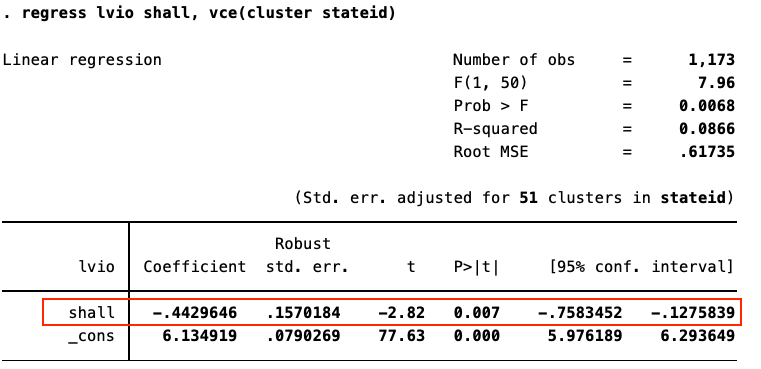
\includegraphics[width=0.9\linewidth]{pictures/Ex1-pooledsimple} \end{center}
\end{frame}

\begin{frame}{Exercise 1(a-ii)
\footnotesize \protect\hyperlink{Ex1-pooledOLS-A}{(\textgreater\textgreater back(1a))}
\normalsize }
\protect\hypertarget{Ex1-pooledwithctrls}{}
\begin{center}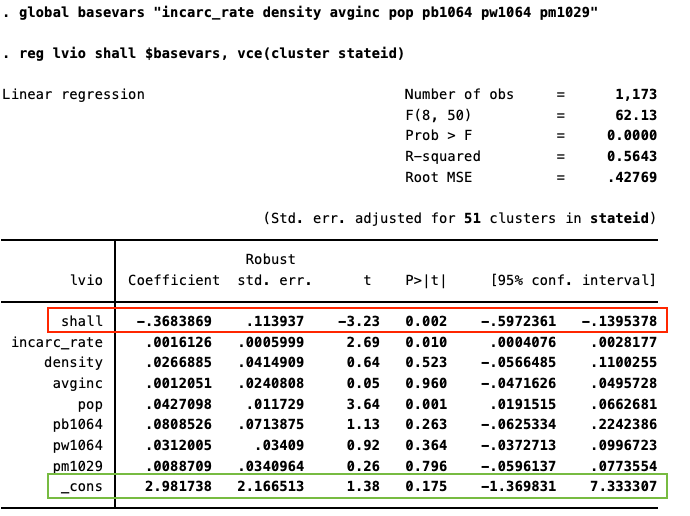
\includegraphics[width=0.9\linewidth]{pictures/Ex1-pooledwithctrols} \end{center}
\end{frame}

\begin{frame}[fragile]{Exercise 1(b-i)}
\protect\hypertarget{Ex1-EntityFEs}{}
\footnotesize

\begin{Shaded}
\begin{Highlighting}[]
\NormalTok{*}\KeywordTok{xtreg}\NormalTok{ yvar xvar, }\KeywordTok{fe} \KeywordTok{vce}\NormalTok{(}\KeywordTok{cluster}\NormalTok{ entityid)}
\end{Highlighting}
\end{Shaded}

\begin{flushleft}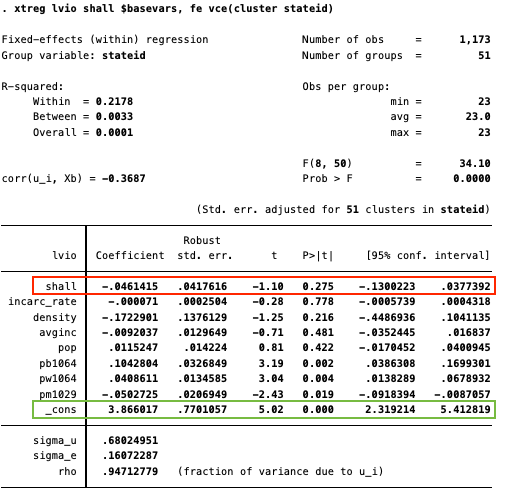
\includegraphics[width=0.8\linewidth]{pictures/Ex1-EntityFEs} \end{flushleft}
\end{frame}

\begin{frame}[fragile]{Exercise 1(b-ii-I)}
\protect\hypertarget{exercise-1b-ii-i}{}
\footnotesize

\begin{Shaded}
\begin{Highlighting}[]
\NormalTok{*}\KeywordTok{xtreg}\NormalTok{ yvar xvar i.timeid, }\KeywordTok{fe} \KeywordTok{vce}\NormalTok{(}\KeywordTok{cluster}\NormalTok{ entityid)}
\end{Highlighting}
\end{Shaded}

\begin{flushleft}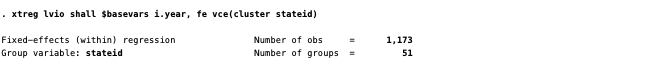
\includegraphics[width=0.95\linewidth]{pictures/Ex1-TwowayFEs-1} \end{flushleft}

\tiny Alternative,

\begin{flushleft}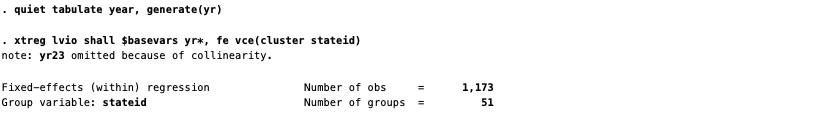
\includegraphics[width=0.95\linewidth]{pictures/Ex1-TwowayFEs-2} \end{flushleft}

\tiny Alternative,

\begin{flushleft}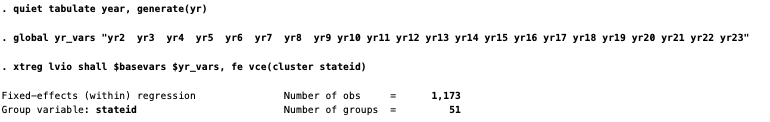
\includegraphics[width=0.95\linewidth]{pictures/Ex1-TwowayFEs-3} \end{flushleft}
\end{frame}

\begin{frame}{Exercise 1(b-ii-II)}
\protect\hypertarget{Ex1-TwowayFEs-4}{}
\begin{flushleft}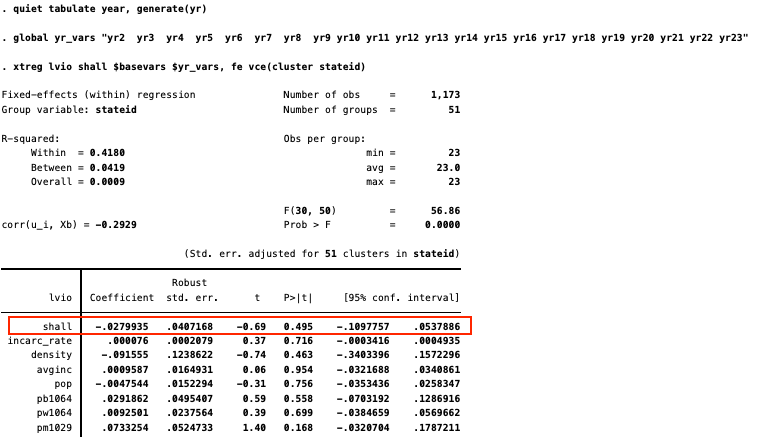
\includegraphics[width=1.05\linewidth]{pictures/Ex1-TwowayFEs-4} \end{flushleft}
\end{frame}

\begin{frame}{Exercise 1(b-iii)}
\protect\hypertarget{Ex1-TestTimeFEs}{}
\begin{flushleft}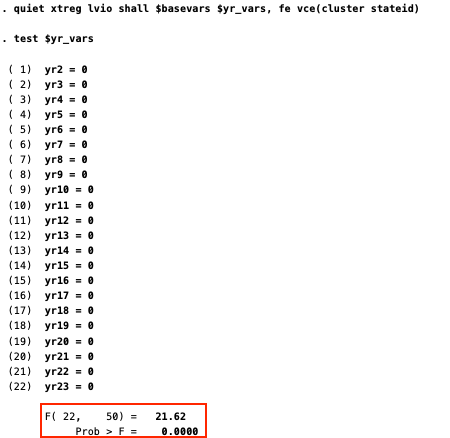
\includegraphics[width=0.7\linewidth]{pictures/Ex1-TestTimeFEs} \end{flushleft}
\end{frame}

\begin{frame}{Exercise 2(b-I)}
\protect\hypertarget{Ex2-pooledsimplewithclustering}{}
\begin{flushleft}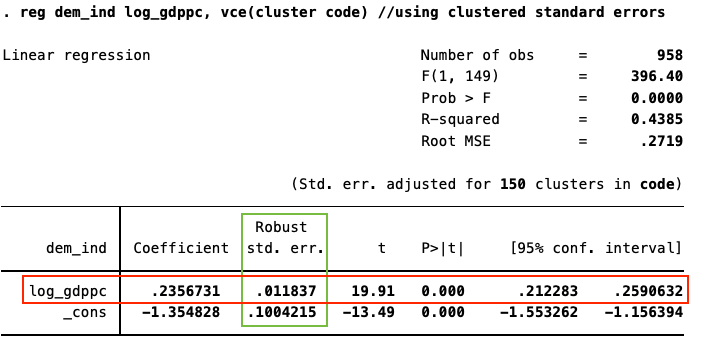
\includegraphics[width=0.9\linewidth]{pictures/Ex2-pooledsimplewithclustering} \end{flushleft}
\end{frame}

\begin{frame}{Exercise 2(b-II)}
\protect\hypertarget{Ex2-pooledsimplemoclustering}{}
\begin{flushleft}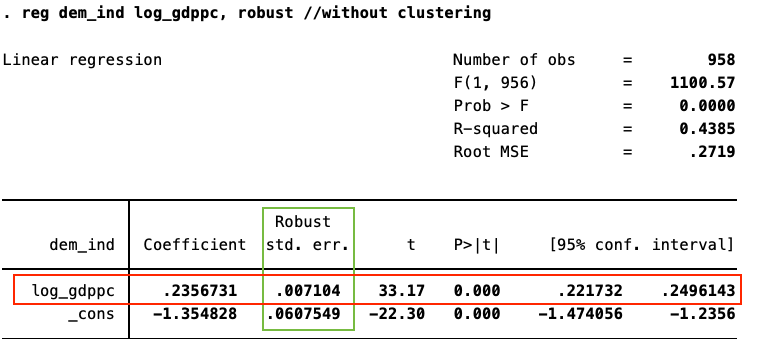
\includegraphics[width=0.9\linewidth]{pictures/Ex2-pooledsimplemoclustering} \end{flushleft}
\end{frame}

\begin{frame}{}
\protect\hypertarget{section-2}{}
\end{frame}

\begin{frame}{}
\protect\hypertarget{section-3}{}
\end{frame}

\begin{frame}{Exercise 2(c)
\footnotesize \protect\hyperlink{Ex2-CountryFEs-A}{(\textgreater\textgreater back(2c))}
\normalsize }
\protect\hypertarget{Ex2-CountryFEs}{}
\end{frame}

\begin{frame}{Exercise 2(d-I)
\footnotesize \protect\hyperlink{Ex2-BothFEs-A}{(\textgreater\textgreater back(2d))}
\normalsize }
\protect\hypertarget{Ex2-BothFEs}{}
\end{frame}

\begin{frame}{Exercise 2(e-II)
\footnotesize \protect\hyperlink{Ex2-BothFEswithcontrols-A}{(\textgreater\textgreater back(2e))}
\normalsize}
\protect\hypertarget{exercise-2e-ii-back2e}{}
\end{frame}

\end{document}
